\documentclass[letterpaper,12pt]{article}   %% LaTeX 2e (preferred)
\usepackage{osajnl2} %% do not use with REVTeX4
\usepackage[draft]{hyperref} %% optional
%%\usepackage{subfigure}
\usepackage{graphicx}
%%\usepackage{caption}
%%\usepackage{subcaption}
%\usepackage{setspace}
%\doublespacing


\begin{document}

\title{Robust self-tuning algorithm for phase shifting interferometry; an improvement 
to the advanced iterative algorithm}

\author{O. Medina,$^{1,*}$ J. C. Estrada,$^{1}$ and M. Servin,$^{1}$}

\address{$^1$Centro de Investigaciones en Optica A. C., Loma del bosque 115, Col. Lomas 
del Campestre, Leon Guanajuato, 37150, Mexico}

\address{$^*$Corresponding author: orlandomedina@cio.mx}

\maketitle

\begin{abstract}
In this work, we develop a regularization technique to demodulate a  phase-shifting 
interferometry sequence with arbitrary inter-frame phase shifts. With this method, 
we can recover the modulating phase and inter-frame phase shifts in the same process. 
As all phase-shifting algorithms, the assumption is that the wave front under test does 
not change over time, but in this case the introduction of phase-shifts can vary in a 
non constant way. Another feature of this demodulation method is that it is able to find 
the modulated phase from interferograms with poor visibility since they have non 
constant background illumination and contrast in their fringes. This advantage is a 
significant improvement to the already published method Advanced Iterative Algorithm (AIA), 
which is sensible to variations in the background illumination and contrast. To see the 
performance of the demodulation technique developed herein, we will show numerical 
experimental results and comparisons with the AIA method.
\end{abstract}
\ocis{120.0120, 120.3180, 120.3940, 120.5050, 120.2650, 050.5080}

\section{Introduction}
Nowadays, Phase Shifting Interferometry (PSI) techniques are some of the most used 
techniques in optical metrology \cite{a1_OpticalTesting}. In PSI, one obtains an small 
sequence of at least 3 interferograms with a phase-shift among them 
\cite{a1_OpticalTesting}. To recover the modulating phase, there are standard 
demodulation PSI methods, the well known 3-, 4-, and 5- step phase-shifting algorithms. 
Knowing the inter-frame phase-shifts (or temporal carrier), the standard methods recover 
the 2$\pi$ modulus phase map with the minimum possible error 
\cite{a1_OpticalTesting,a2_F&K,a3}. If we do not know the phase-shifts exactly, we obtain 
a phase map with an unavoidable detuning error whose magnitude depends on the number of 
interferograms employed and on how far we are from the actual phase-shifts 
\cite{a3,a4,a5,a6}. This unfortunate case can occur when the optical interferometer setup 
is uncalibrated or when perturbations from the environment affect the interferometer's 
optical path. For example, for most phase shifters, such as a piezoelectric (PZT), there 
is a repeatability problem arising from hysteresis, non linearity and temperature linear 
drift \cite{a5,a7}; curiously, the first phase-shifting algorithms were self-tuning 
nonlinear algorithms \cite{a8,a9}. To reduce detuning errors, other approaches propose 
error compensating algorithms that basically use redundant data, such as the Schwider-
Hariharan 5- step algorithm, \cite{a4,a10,a11} and more recently, the 9-step algorithm 
shown in Ref. \cite{a12} has been used to do it by constructing a wide-band frequency 
response of the phase-shifting algorithm. Further methods use the Fourier transform in 
order to estimate the inter-frame phase-shifts, and others are based on the least-squares 
scheme, iteratively estimating the inter-frame phase-shifts and phase \cite{a13,a14}. 
Ref. \cite{a16} presentes an approach that estimates the local temporal carrier (the 
phase-shift) as the average of the phase difference between two consecutive phase maps 
obtained from two realizations of the tunable 3-step algorithm. What we are going to show 
in this work is a regularized self-tuning demodulation technique that obtains the 
analytical image (complex interferogram) and inter-frame phase-shifts from an 
interferogram sequence. Thus, we can recover the modulating phase 2$\pi$ modulus and the 
inter-frame phase shifts in the same process. Here, it is not necessary to know the 
inter-frame phase-shifts. These inter-frame phase-shifts can vary arbitrarily.

The main difference between the demodulation method presented here and the ones reported 
in  \cite{a14},\cite{a15} and \cite{a17} is that our demodulation method is based on a 
regularization technique that is robust to non constant modulation variations and non 
constant background illumination, which is an issue that introduces errors in the methods 
in works \cite{a14} and \cite{a15}. Besides, we do not require to estimate the fringe 
orientation, as the method in work \cite{a17}.

\section{Method}

In general, an interferogram sequence with arbitrary inter-frame phase-shifts can be
modeled as:
\begin{equation}\label{I_k1}
	I_{x,y}^k=a_{x,y}+b_{x,y}cos(\phi_{x,y}+\alpha_k),\: k=0,1,2,...,L-1,
\end{equation}
where $I_{x,y}^k$ is the intensity at the site $x,y$ of the $k$-interferogram in a 
sequence of $L-1$ interferograms, being $a_{x,y}$ its background illumination, $b_{x,y}$
its contrast, $\phi_{x,y}$ the modulating phase under test and $\alpha_k$ the phase-shift
of the $k$-interferogram.

\subsection{Least-squares method}

As we can see from Eq. (\ref{I_k1}), conventional phase-shifting algorithms assumes that
the background illumination and the modulation amplitude do not have frame-to-frame
variation; i.e., they are functions of pixels only. Defining a new set of variables as
$\varphi_{x,y}=b_{x,y}cos(\phi_{x,y})$, $\psi_{x,y}=b_{x,y}sin(\phi_{x,y})$,
$C_k=cos(\alpha_k)$, $S_k=sin(\alpha_k)$ we can express Eq. (\ref{I_k1}) as
\begin{equation}\label{I_k2}
	I_{x,y}^k=a_{x,y}+\varphi_{x,y}C_k-\psi_{x,y}S_k,\: k=0,1,2,...,L-1.
\end{equation}
If we known $\alpha_k$, there are $3MN$ unknowns (where $M$ and $N$ are the interferogram
dimension). These unknowns can be solved using least-squares method. An energy cost 
function that described above can be written as
\begin{equation}\label{ls_funtional}
	U(a_{x,y},\varphi_{x,y},\psi_{x,y})=\sum_{k=0}^{L-1}
	[a_{x,y}+\varphi_{x,y}C_k-\psi_{x,y}S_k-I_{x,y,k}^{'}]^2,
\end{equation}
where $I_{x,y,k}^{'}$ is the $k$-th experimentally measured intensity of the 
interferogram sequence. For the known $\alpha_k$, the least-squares criteria require to 
make zero the gradient of Eq. (\ref{ls_funtional}) as
\begin{equation}\label{minimize_U}
	\nabla U(a_{x,y},\varphi_{x,y},\psi_{x,y})=0.
\end{equation}
Eq. (\ref{minimize_U}) yield
\begin{equation}\label{x=AB}
	X = A^{-1} B,
\end{equation}
where
\begin{equation}\label{A}
	A = \left[ \begin{array}{c c c}
	M\times N & \sum C_k     & \sum S_k \\
	\sum C_k  & \sum C_k^2   & \sum C_k S_k \\
	\sum S_k  & \sum S_k C_k & \sum S_k^2\end{array} \right],
\end{equation}

\begin{equation}\label{B}
	B = \left[ \begin{array}{c c c}
	\sum I_{x,y,k}^{'} & \sum I_{x,y,k}^{'} C_k & \sum I_{x,y,k}^{'} S_k \end{array}
	\right]^T,
\end{equation}

\begin{equation}\label{X}
	X = \left[ \begin{array}{c c c}
	a_{x,y} & \varphi_{x,y} & \psi_{x,y} \end{array} \right]^T,
\end{equation}
where the sum $\sum$ runs over $k=0,1,2,...,L-1$. To ensure that $A$ is nonsingular Eq.
(\ref{x=AB}) requires at least three different phase-steps $\alpha_k$. From Eqs.
(\ref{A})-(\ref{X}) the phase $\phi$ at the point $x,y$ can be determined from
\begin{equation}
	\phi_{x,y} = \arctan(-\psi_{x,y}/\varphi_{x,y}).
\end{equation}
Note that the inverse of A is performed only once because its components depend only on
the steps $\alpha_k$.

%%---------------------------------------------------------------------------
\subsection{Robust self-tuning (RST) method}
\begin{figure}[th]
	\begin{center}
		\begin{tabular}{ c c c c c }
			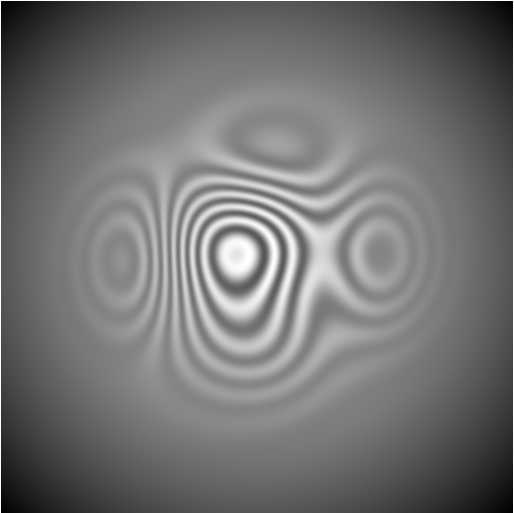
\includegraphics[scale=0.20]{figures/Interferograma.png} }&
			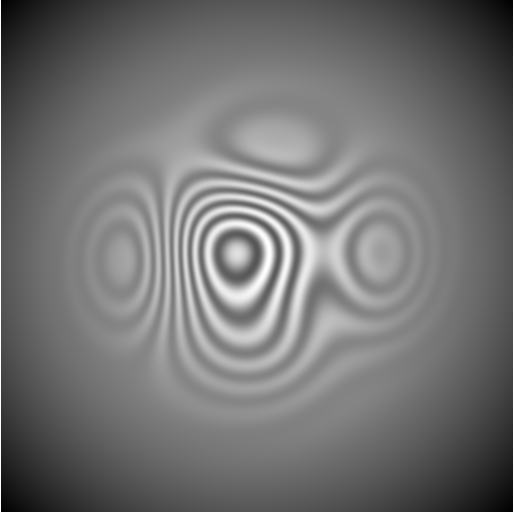
\includegraphics[scale=0.20]{figures/Interferograma2.png}}&
			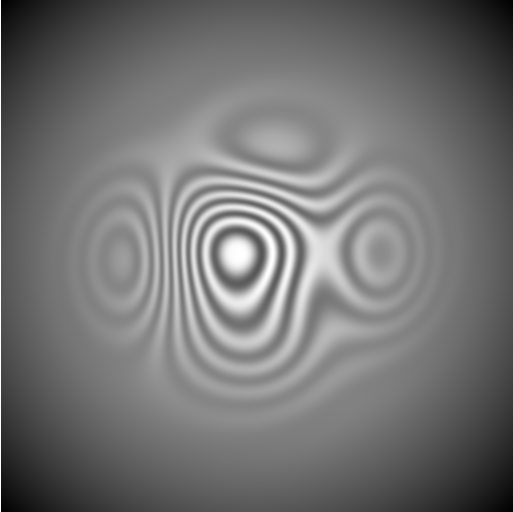
\includegraphics[scale=0.20]{figures/Interferograma3.png}}&
			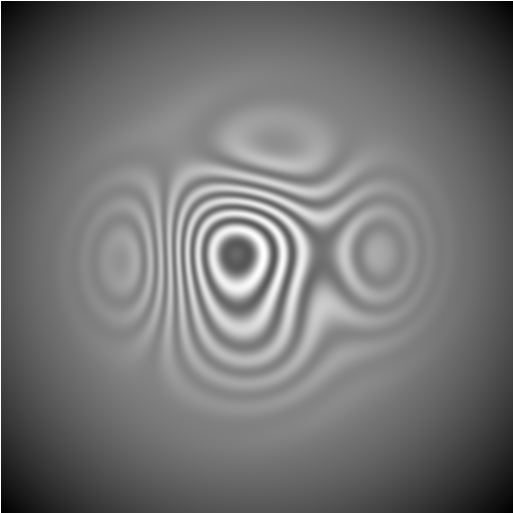
\includegraphics[scale=0.20]{figures/Interferograma4.png}}&
			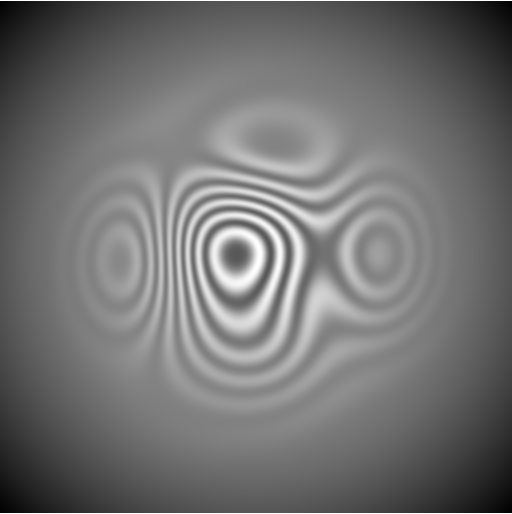
\includegraphics[scale=0.20]{figures/Interferograma5.png}}& \\
		  	I_0 &  I_1 & I_2 &  I_3 &  I_4
		\end{tabular}	
	\end{center}
	\caption{Interferogram sequence used for testing the AIA and proposed algorithm 
	(RST).} 
	\label{fig:Interferograms}
\end{figure}
To determine the steps we propose the following regularized cost functional
\begin{eqnarray} \label{rst_functional}
	\left U(a_{x,y},C_{x,y}^k,S_{x,y}^k) & = & \sum_{x,y} \sum_{k=0}^{L-1}
	\sum_{m=-1}^{1} \sum_{n=-1}^{1}
	\left[a_{x,y}+\varphi_{x+m,y+n}C_{x,y}^k-\psi_{x+m,y+n}S_{x,y}^k-I_{x+m,y+n,k}^{'}
	\right] ^2 \nonumber \\
	& & {} + \sum_{x,y} \sum_{k=0}^{L-1} \left[ \lambda \frac{\nabla[a_{x,y}]}{L} +
	\mu \nabla[C_{x,y}^k] + \mu \nabla[S_{x,y}^k] \right] ^2,
\end{eqnarray}
where $\lambda$ and $\mu$ are the regularization parameters that controls the smoothness
of $a_{x,y}$, $C_{x,y}^k$ and $S_{x,y}^k$. Operator $\nabla[*]$ takes the first order
differences along $x$ and $y$ direction, as follows:
\begin{equation}
	\nabla[f_{x,y}] = [a_{x,y}-a_{x-1,y},a_{x,y}-a_{x,y-1}]^T.
\end{equation}

To find our unkown steps we need to minimize the cost functional in Eq 
\ref{rst_functional}. Equating to zero the partial gradient with respect to $a_{x,y}$, 
$C_{x,y}^k$ and $S_{x,y}^k$ and solving, we obtain a closed formula for iterative 
computing the background illumination and the phase-shift steps, as follows:
\begin{equation}
	a_{x,y} = \frac{ \sum_{k=0}^{L-1} \sum_{m=-1}^{1} \sum_{n=-1}^{1} \left[\\
	-\varphi_{x+m,y+n}C_{x,y}^k+\psi_{x+m,y+n}S_{x,y}^k+I_{x+m,y+n,k}^{'} \right] }
	{ 9L - a_{x-1,y}-a_{x,y-1}},
\end{equation}
\begin{equation}\label{C_xy}
	C_{x,y}^k = \frac{ \sum_{m=-1}^{1} \sum_{n=-1}^{1} \left[ -a_{x,y} \varphi_{x+m,y+n}+
	\psi_{x+m,y+n} \varphi_{x+m,y+n} S_{x,y}^k +\\ 		I_{x+m,y+n,k}^{'}
	\varphi_{x+m,y+n} \right] } { \sum_{m=-1}^{1} \sum_{n=-1}^{1} \varphi_{x+m,y+n}^2 -
	C_{x-1,y}^k-C_{x,y-1}^k },
\end{equation}
\begin{equation}\label{S_xy}
	S_{x,y}^k = \frac{ \sum_{m=-1}^{1} \sum_{n=-1}^{1} \left[ a_{x,y} \psi_{x+m,y+n} +
	\psi_{x+m,y+n} \varphi_{x+m,y+n} C_{x,y}^k-I_{x+m,y+n,k}^{'} \psi_{x+m,y+n} \right]}
	{ \sum_{m=-1}^{1} \sum_{n=-1}^{1} \psi_{x+m,y+n}^2 - S_{x-1,y}^k - S_{x,y-1}^k }.
\end{equation}
As we see from Eqs \ref{C_xy} and \ref{S_xy} we can comput the phase-shift in every site
of each interferogram. Then to obtain the phase-shift steps
\begin{equation}
	\alpha_k = \arctan(-S_m^k/C_m^k),
\end{equation}
where $S_m^k$ and $C_m^k$ are the mode, most frequent value, calculated for each
interferogram.
Now, to determine the modulated phase we use the least squares method and the proposed
method alternately until the values ​​of the phase-shifts converge to a desired value.

%% ------------------------------------- Resultados ----------------------------
\section{Numerical Experiments and Results}
\begin{figure}[ t]
	\begin{center}
		\begin{tabular}{c c}
			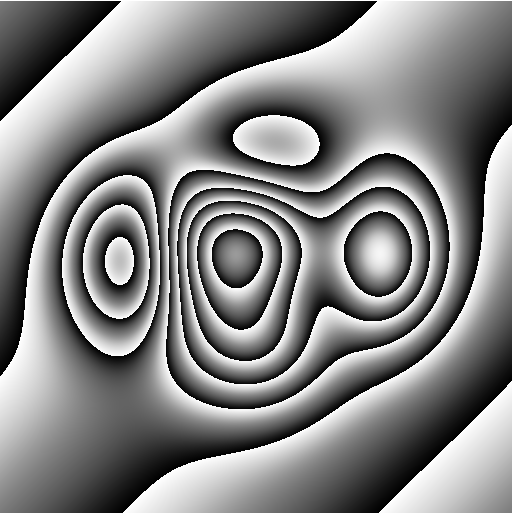
\includegraphics[scale=0.35]{figures/faseRST.png}}&
			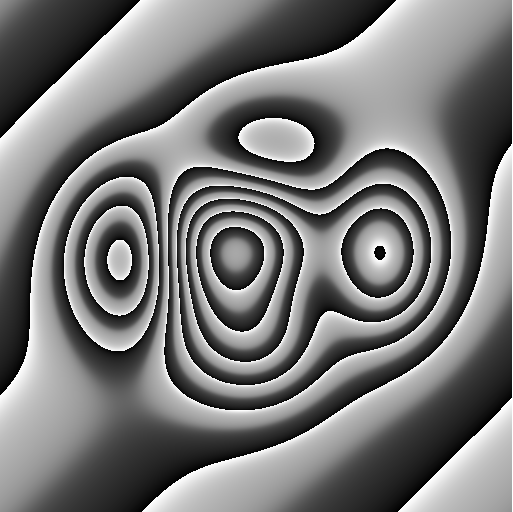
\includegraphics[scale=0.35]{figures/faseAIA.png}}& \\
			(a) RST Phase error =  7.0570x10^{-06}. & (b) AIA Phase error =  0.0608
		\end{tabular}
	\end{center}
	\caption{Phase Comparison.(a) shows the recovered phase and error using the
	regularized self-tuning (RST) method proposed here. (b)  shows the recovered phase
	and error using the AIA method. The error shown (in radians) is the variance
	respecting the true phase map. The interferogram frames has a size of 512 x 512.}
	\label{fig:phase}
\end{figure}

To test the robust self tuning algorithm developed here, we simulated $50$ interferogram
sequences with different temporal frequecies. Each sequence has five interferograms. An
example of these interferogram sequences is shown in Fig.\ref{fig:Interferograms}. These
simulated interferograms have poor fringe visibility since we have added a non constant
background illumination and contrast.  To reproduce the interferogram sequences that we
used in these tests, the reader can use the Eq. \ref{I_k1} with the following parameters:
\begin{equation}
	a_{x,y}=-\frac{(x-256)^2+(y-256)^2}{1.5259x10^{-5}},
\end{equation}
\begin{equation}
	b_{x,y}=e^{-\frac{(x-256)^2+(y-256)^2}{100^{2}}},
\end{equation}
\begin{equation}
	\phi_{x,y}= 30(-1+\frac{x}{2}-x^5-y^3) e^{(-x^2-y^2)}+\frac{4\pi x}{512}+\frac{4\pi
	 y}{512},
\end{equation}
and
\begin{equation}
	\alpha_k = k\frac{\pi}{3}+\eta_k,\: k=0,1,..,5,
\end{equation}
where $\eta_k$ is a random number with mean zero and variance of 0.5 that changes at 
each step.
In our numerical experiments we start always the temporal carrier $\alpha_k=0,1,..,5$.
Regularization parameters $\lambda$ and $\mu$ were set at 100 and 500 respectively (see 
Eq. \ref{rst_functional}). Using the Gauss-Seidel method to find the phase-steps (Eqs. 
13, 14 and 15) were required 50 iterations. Finally, for estimating the phase in the AIA 
and our proposed method were required 20 iterations.

In Table. \ref{Tab:step-error} , we show the errors values of the estimated phase-shifts 
using our regularized method and the estimated using the AIA method. This errors are 
calculated as $|\alpha_k - \hat{ \alpha }_k }|$, where $\alpha_k$ and $\hat{\alpha}_k$ 
are the values of the actual and estimated phase-shifts for the $k-$frame, respectively. 
On the other hand, in Fig. \ref{fig:phase} , we show the recovered phase. In Fig. 
\ref{fig:phase}(a) is shown the recovered phase using the regularized self-tuning 
demodulation method presented here, while in Fig. \ref{fig:phase}(b) is shown the 
recovered phase using the AIA method.
We can see in this figure that our proposed regularized self-tuning demodulation method
recovers the phase with less error than with the AIA method. The errors shown in Fig.
\ref{fig:phase}(a) and Fig. \ref{fig:phase}(b) are calculated as the variance between 
the recovered phase map and the true phase map used to generate the interferograms.
\begin{table}[h t p]
	\begin{center}
		\begin{tabular}{|c|c|c|c|}
		\hline
		 Steps   & Actual & AIA    & RST 	\\ \hline \hline
		\alpha_0 & 	0	  & 0 	   & 0		\\ \hline
		\alpha_1 & 1.6953 &	2.2511 & 1.6994	\\ \hline
		\alpha_2 & 0.6961 &	0.6284 & 0.6769	\\ \hline
		\alpha_3 & 3.3038 &	3.2427 & 3.3031	\\ \hline
		\alpha_4 & 4.0793 &	4.2983 & 4.0678	\\ \hline
		e^{ave}  &        & 0.1807 & 0.0071 \\ \hline
		\end{tabular}
	\end{center}
	\caption{Numerical results. Comparison between the phase-shift estimation and the
	 actual phase-shift for the AIA and the proposed method, and the phase-shift 
	 average error.} 
	\label{Tab:step-error}
\end{table}

On the other hand, Table 2 shows the average error of 50 random tests, with the same 
parameters listed above. As seen from these results, the proposed method recovers the
stage with three orders of magnitude less than the AIA method.
Finally, in Fig 3(b) shows the recovered phase with the RST method using a 4-frame
experimental sequence. The interferogram shown in Fig 3 (a) is the first frame of the 
sequence used. For demonstration purposes, we modify the contrast and backlight of the 
original experimental sequence as follows: $I_n=a+bI$, where $a$ is a parabola centered 
at the origin with amplitude of one and $b$ is a Gaussian with variance 7.
\begin{table}
	\begin{center}
		\begin{tabular}{|l|c|c|}
		\hline
		            & AIA    & RST 	    \\ \hline \hline
		Step-error  & 0.1902 & 0.0153	\\ \hline
		Phase-error & 4.57x10^{-2} & 5.11x10^{-5} \\ \hline
		\end{tabular}
	\end{center}
	\caption{This table compares the average error obtained in 50 random tests for the
	proposed method and the AIA method. The first row shows the average error of
	estimated steps, while the second shows the variance between the estimated phase map
	and the used to generate the sequence of interferograms.} 
	\label{Tab:mean-phase_error}
\end{table}
\begin{figure}[h t]
	\begin{center}
		\begin{tabular}{c c}
			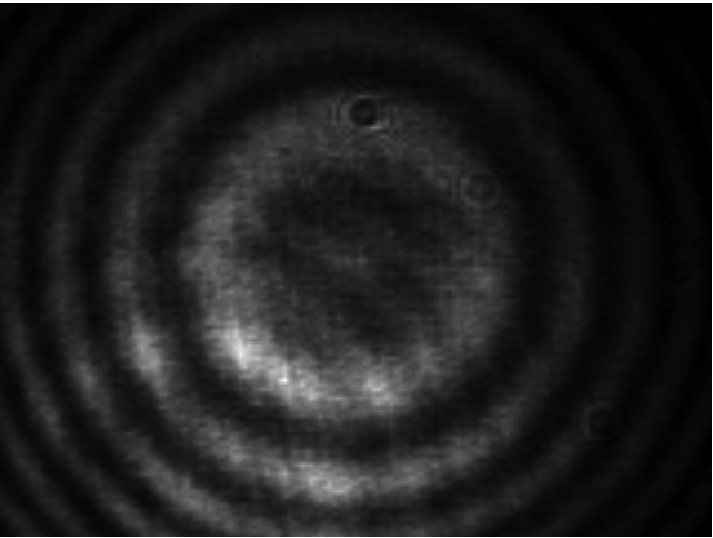
\includegraphics[scale=0.35]{figures/InterferogramaExpMod.png}}&
			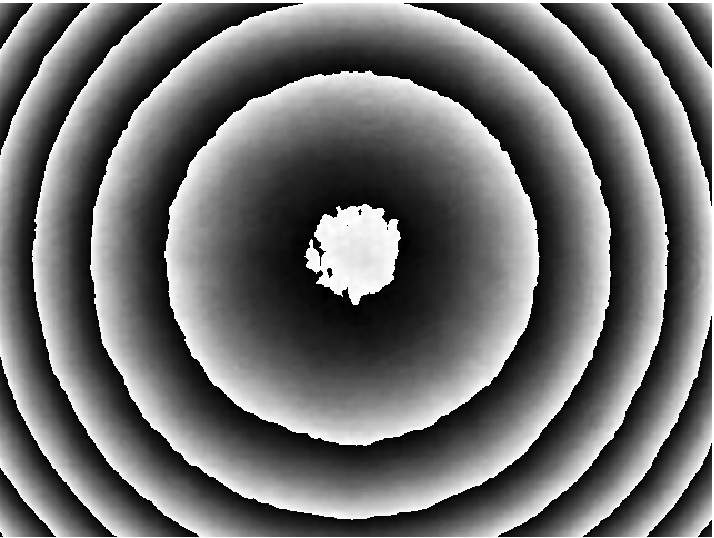
\includegraphics[scale=0.35]{figures/faseExpRST.png}}& \\
			(a) Experimental Interferogram. & (b) Recovered phase map
		\end{tabular}
	\end{center}
	\caption{Experimental test.(a) Shows an experimental interferogram with background 
	illumination and contrast modifed. (b) Shows the recovered phase map using the RST 
	method.}
	\label{fig:ExpPhase}
\end{figure}


%%----------------------------- Conclusiones ------------------------------------
\section{Conclusions}

We have presented a regularized self-tuning phase-shifting demodulation method for 
interferogram sequences having arbitrary variations of the inter-frame phase-shifts. 
This method is robust to non constant background illumination. As shown in the results,
our demodulation method is able to recover the modulating phase and the inter-frame 
phase-shifts with a minimum error. The demodulation method presented here provides 
stable convergence and accurate phase demodulation with as few as three interferograms,
even when the phase-shifts are completely random.

\bibliographystyle{plain}
\bibliography{rst.bib}
\end{document}
